% !TEX options=--shell-escape
\documentclass[usenames,dvipsnames,9pt]{beamer}

\makeatletter
\def\input@path{{support/beamer-template/}}
\makeatother

\usepackage{support/beamer-template/beamerthememetropolis}

\usepackage[utf8]{inputenc}
\usepackage[czech]{babel}
\selectlanguage{czech}

\usepackage{hyperref}
\usepackage{fontawesome}
\usepackage{minted}
\usepackage{mathtools}
\usepackage{tabularx}
\usepackage{smartdiagram}
\usepackage{soul}
\usepackage{tikz}
\usepackage{amssymb}
\usepackage{qrcode}

% Commands shared between most of the tutorial slides

% Homework deadlines
\newcommand{\hwVIIdeadline}{10. 5. 2020}



% Download icon and text with link relative to the root of the courseware site
\newcommand{\download}[1]{\hfill\faDownload\hspace{5pt}\href{https://cw.fel.cvut.cz/wiki/_media/courses/be4m36mas/#1}{\tt #1}\\[1.3em]}

% Draw eye icon
\newcommand{\see}[1]{\faEye\hspace{5pt}#1}

\newcommand{\sep}{\hspace{10pt}/\hspace{10pt}}

\def\Ipe#1{\def\IPEfile{#1}\input{#1}}

% Draw pacman icon
\newcommand{\pacman}[1]{\tikz[baseline=.1em,scale=.6]{
    \useasboundingbox (.02,0) rectangle (.6,.6);
  \draw [fill=#1] (.3,.3) -- ++(25:.3) arc (+25:+335:.3) -- cycle;

}}

% Draw ghost icon
\newcommand{\ghost}[1]{\tikz[baseline=.1em,scale=.5]{
  \draw [fill=#1] (0,0) -- (0,.5) arc (+180:0:.3) -- (.6,0) --
  (.5,.15) -- (.4,0) -- (.3,.15) -- (.2,0) -- (.1,.15) -- cycle;
    \coordinate (eye) at (360*rand:.03);
    \foreach \x in {.17,.43}{
      \fill[white] (\x,.5) circle[radius=.1];
      \fill[black] (\x,.5) ++(eye) circle[radius=.05];
    }
}}

\newcommand{\desc}[2]{
  #1

  \vspace{-0.6em}
  \hfill\begin{minipage}{0.9\linewidth}
    #2
  \end{minipage}

  \vspace{0.2em}
}

\newcommand{\redc}{\tikz\draw[red,fill=red] (0,0) circle (.5ex);}

\newcommand{\greenc}{\tikz\draw[green,fill=green] (0,0) circle (.5ex);}


% Default url for generating QR code with feedback form.
\newcommand{\defaultfeedbackurl}{https://forms.gle/vwbWazEu14w1Kf487}

% Generate frame with QR code to a feedback form.
\newcommand{\framefeedback}[1][\defaultfeedbackurl]{
  \begin{frame}[standout]
    \begin{minipage}{0.4\linewidth}
      \begin{center}
        \textbf{\LARGE Díky za pozornost!}
      \end{center}

      \vspace{3em}

      \raggedleft\small Budeme rádi za Vaši\\zpětnou vazbu! $\rightarrow$
    \end{minipage}
    \hfill
    \begin{minipage}{0.5\linewidth}
      \vspace{4em}
      \centering\qrcode[height=\linewidth]{#1}\\
      \vspace{0.8em}
      \url{#1}
    \end{minipage}
  \end{frame}
}

\title{Vektorové instrukce}
\date{\today}
\institute{B4B36PDV -- Paralelní a distribuované výpočty}

\metroset{block=fill}

\begin{document}
\maketitle

\begin{frame}
  \frametitle{Osnova}
  \begin{itemize}
    \item Opakování z minulého cvičení\\[1.5em]
    \item Autovektorizace
    \item Ruční vektorizace pomocí intrinsics\\[1.5em]
    %\item Zadání semestrální úlohy
  \end{itemize}
\end{frame}


\section{Opakování z minulého cvičení}

\begin{frame}[standout]
  \Huge
  \url{http://goo.gl/a6BEMb}
\end{frame}

{\setbeamertemplate{frame footer}{\see{\url{http://goo.gl/a6BEMb}}}
\begin{frame}[fragile]
\frametitle{Který způsob je efektivnější?}

 \begin{minted}{c}
bool mat[M][N];

// A:
#pragma omp parallel
#pragma omp for
for(int i = 0; i < M; i++) {
 for(int j = 0; j < N; j++){
    if (mat[i][j]){ /* report solution and terminate all; */ }
}}

// B:
for(int i = 0; i < M; i++) {
  #pragma omp parallel
  #pragma omp for
  for(int j = 0; j < N; j++){
    if (mat[i][j]){ /* report solution and terminate all; */ }
}}
 \end{minted}

\end{frame}

\begin{frame}[fragile]
\frametitle{Jakým způsobem bude následující kód proveden?}

 \begin{minted}{c}
bool mat[M][N];
for(int i = 0; i < M; i++) {
    #pragma omp parallel
    #pragma omp for
    for(int j = 0; j < N; j++){
        #pragma omp cancellation point for
        if (mat[i][j]){
            #pragma omp cancel for
        }
    }
}
std::cout << "Finished!" << std::endl;
 \end{minted}
 
 \vspace{.3em}
 
 \begin{itemize}
 \item Výpočet končí okamžitě po nalezení prvního řešení.
 \item Po nalezení prvního řešení výpočet skončí, až všechna vlákna narazí na 'cancellation point'.
 \item Ani jedna z předchozích odpovědí není správná.
 \end{itemize}

\end{frame}



}

\begin{frame}[t]
  \frametitle{Moderní procesor}
  \centering
  \smartdiagram[bubble diagram]{Paralelizace,
    Pipelining \\ {\footnotesize (procesor)},
    Vektorizace \\ {\footnotesize (kompilátor)},
    Vlákna \\ {\footnotesize (Vy :-)}}
\end{frame}

\begin{frame}[t]
  \frametitle{Moderní procesor}
  \centering
  \smartdiagram[bubble diagram]{Paralelizace,
    Pipelining \\ {\footnotesize (procesor)},
    Vektorizace \\ \st{\footnotesize (kompilátor)} \\ \textcolor{BrickRed}{\bf (Vy :-)},
    Vlákna \\ {\footnotesize (Vy :-)}}
\end{frame}

\begin{frame}
  \frametitle{Skalární zpracování dat}
  \begin{center}
    
\includegraphics[width=0.4\linewidth]{07/figs/scalar.pdf}
  \end{center}
\end{frame}

\begin{frame}
  \frametitle{Vektorové zpracování dat}
  \begin{center}
    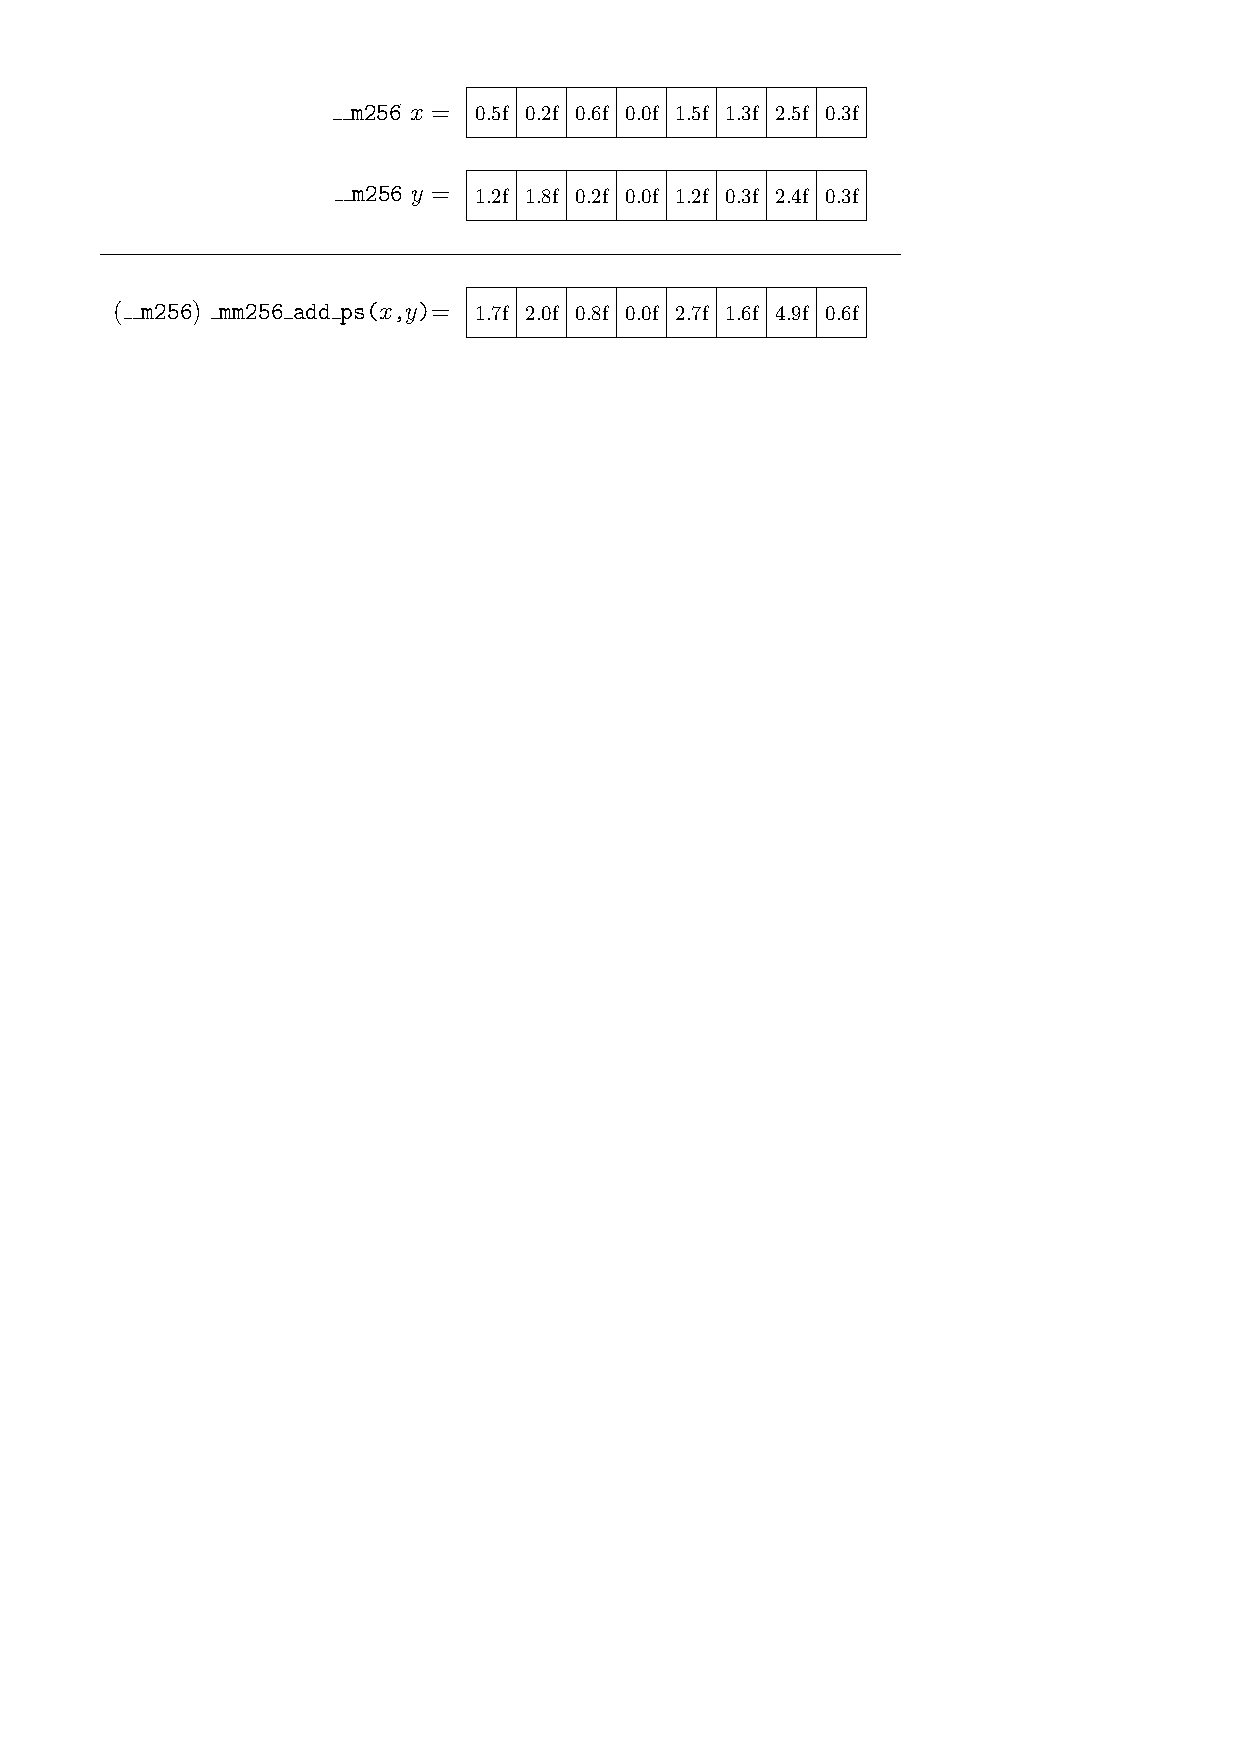
\includegraphics[width=0.95\linewidth]{07/figs/vectorized.pdf}
  \end{center}
  \pause
  \vspace{1.5em}
  \begin{center}
    \LARGE Není to až taková magie, jak to vypadá :-)
  \end{center}
\end{frame}

\begin{frame}
  \frametitle{Vektorové zpracování dat (pomocí AVX / AVX2)}

  \hfill \texttt{\#include <immintrin.h>}
  \vspace{1em}

  \begin{itemize}
    \item {\large \texttt{\_\_m256} - datový typ ,,vektor délky 256 bitů``} \\
          \hspace{30pt}(\texttt{float} má 32 bitů, a proto se do takového vektoru vejde 8x)
    \pause
    \item {\large \texttt{\_mm256\_add\_ps($x$,$y$)}}
          \begin{itemize}
            \item Nad dvěma 256-bitovými vektory $x$ a $y$... (\texttt{\_mm256\_})
            \item ...provádím operaci sčítání... (\texttt{add})
            \item ...při čemž vektory obsahují elementy typu \emph{packed-single} (\texttt{\_ps}).
          \end{itemize}
    \pause
    \vspace{1em}
    \item \emph{packed} -- vektor ,,zabaluje`` více prvků stejného typu
    \item \emph{single} -- \emph{single-precision number} aka \texttt{float}
  \end{itemize}
\end{frame}

\begin{frame}[fragile]
  \begin{center}
    \LARGE\bf Level 1: Autovektorizace \hspace{10pt} \ghost{yellow!85!red}
  \end{center}
\end{frame}

\begin{frame}[fragile]
  Moderní kompilátor se snaží zdetekovat \texttt{for} smyčky, které lze vektorizovat...

  Například:

  \begin{minted}{c}
    float a[1024], b[1024], c[1024];
    for(int i = 0 ; i < 1024 ; i++) {
      a[i] = b[i] + c[i];
    }
  \end{minted}

  lze převést na

  \begin{minted}{c}
    for(int i = 0 ; i < 1024 ; i += 8) {
      _mm256_storeu_ps(&a[i],
        _mm256_add_ps(
          _mm256_loadu_ps(&b[i]),
          _mm256_loadu_ps(&c[i])
      ));
    }
  \end{minted}
\end{frame}

\begin{frame}
\frametitle{Autovektorizace GCC}

Vektorizaci kontrolujeme s pomocí parametrů kompilátoru:

\begin{itemize}
    \item \texttt{-march=native}: zapne kompilaci přímo na konrétní hw, včetně zpřístupnění vektorových instrukcí.
    \item \texttt{-ftree-vectorize}: zapne autovektorizaci.
    \item \texttt{-fopt-info-vec-all}: informace o autovektorizaci.
    \item \texttt{-O2} musíme snížit level optimalizace, abychom mohli kontrolovat autovektorizaci.
\end{itemize}

\end{frame}


\begin{frame}
\frametitle{Autovektorizace MSVC}

Vektorizaci kontrolujeme s pomocí parametrů kompilátoru \textbf{a přímo ve zdrojovém kódu}. Vektorizace je na úrovni \texttt{/O2} defaultně zapnutá.

\begin{itemize}
    \item \texttt{/Qvec-report:2}: informace o autovektorizaci.
    \item \texttt{/fp:fast} zpřístupní pokročilou autovektorizaci floatů, která ale může mít vliv na výsledek (float operace na počítačích nejsou komutativní...).
    \item \texttt{\#pragma loop(no\_vector)}: Deaktivuje autovektorizaci pro konkrétní cyklus.
\end{itemize}
    
\end{frame}

{\setbeamertemplate{frame footer}{\exe{{\tt autovec[.exe]}}}
\begin{frame}
  \begin{block}{Vyzkoušejte si autovektorizaci}
    Spusťte autovec(.exe) s autovektorizací a následně zkuste autovektorizaci vypnout:
    \begin{enumerate}
      \item {\Large\textbf{GCC}}: zakomentujte v souboru \texttt{CMakeLists.txt} řádek \texttt{add\_compile\_options("-ftree-vectorize")}
      \item {\Large\textbf{MSVC}}: v souboru \texttt{autovec.cpp} odkomentujte v metodě \texttt{runSequential} řádek \texttt{\#pragma loop(no\_vector) }.
    \end{enumerate}
    Jak se program zpomalí, pokud vypnete autovektorizaci?
  \end{block}
  Také se podívejte do logu ze sestavování programu na zprávy o proběhlé autovektorizaci.
  
   {\small
  Kódy pro důvod selhání autovektorizace v MSVC: \url{https://docs.microsoft.com/en-us/cpp/error-messages/tool-errors/vectorizer-and-parallelizer-messages}}
  
\end{frame}
}

\begin{frame}[fragile]
  \begin{itemize}
    \item[\LARGE\bf\textcolor{OliveGreen}{+}] Je to ,,zadarmo`` (kompilátor se pokusí vektorizaci provést za Vás) \\[2em]
    \pause
    \item[\LARGE\bf\textcolor{BrickRed}{-}] Ne vždy se to kompilátoru musí povést...
    \pause
    \begin{itemize}
      \item Kompilátor vám nemusí ,,rozumět``\\
            (často dokáže vektorizovat jenom smyčky v určitém tvaru) \\[0.6em]
      \pause
      \item Kompilátor musí zajistit, že výsledek programu bude identický, jako kdyby nevektorizoval \textbf{i za těch nejhorších možných podmínek}
            \begin{itemize}
              \item Musí uvažovat, že může dojít k datovým závislostem
              \item Musí zajistit, že dojde ke \underline{stejnému} zaokrouhlení při floating-point operacích
            \end{itemize}
    \end{itemize}
  \end{itemize}

  \pause
  \vspace{1em}\hrule\vspace{1em}

  \begin{minted}[fontsize=\small]{c}
    float x;
    float y1 = x * x * x * x * x * x * x * x;

    float y2 = x * x;
    y2 = y2 * y2;
    y2 = y2 * y2;

    assert(y1 == y2);
  \end{minted}
\end{frame}

\begin{frame}[fragile]
  \begin{center}
    \LARGE\bf Level 2: Intel SPMD Compiler (a jiné) \hspace{10pt} \ghost{yellow!85!red} \ghost{yellow!50!red}
  \end{center}
\end{frame}

\begin{frame}
  \frametitle{Intel SPMD Compiler (ISPC)}

  \begin{center}
    \LARGE Tušíte co znamená zkratka SPMD?
  \end{center}

  \vspace{1em}\hrule\vspace{1em}

  \textbf{SPMD = \emph{single-program multiple-data}}

  Napíšete jeden program, který ale pomocí vektorizace poběží na více daty současně.
  Kompilátor za vás rozhodne, jak má vektorizace proběhnout.
\end{frame}

\begin{frame}
  \frametitle{Intel SPMD Compiler (ISPC)}

  \textbf{Intel SPMD Compiler (ISPC)}
  \begin{itemize}
    \item Nadstavba jazyka C
    \item Od základu uvažuje o programu jako o \underline{paralelním}!
  \end{itemize}

  \vspace{3em}
  \pause
  \begin{center}
    \LARGE\bf Bohužel nemáme čas se ISPC na PDV věnovat :-(
  \end{center}
\end{frame}

\begin{frame}[fragile]
  \begin{center}
    \LARGE\bf Level 3: Intrinsics \hspace{10pt} \ghost{yellow!85!red} \ghost{yellow!50!red} \ghost{yellow!20!red}
  \end{center}
\end{frame}

\begin{frame}
  \frametitle{Intrinsics}

  {\large \textbf{Intrinsics} -- Funkce a datové typy, které zpřístupňují nativní instrukce procesoru \textbf{bez nutnosti programovat v assembleru}}

  \vspace{1em}

  \hfill{\LARGE\bf Instrukční sada: AVX / AVX2}

  \pause

   \vspace{3em}
   \url{https://intel.ly/2GOHp7r} (Intel Intrinsics Guide)

   \hspace{10pt} Výborná reference! Využívejte, když si nebudete jistí!
\end{frame}

\begin{frame}[standout]
  \texttt{\#include <immintrin.h>} \\[2em]
  \faWarning\ \ \ V GCC je třeba všechny kódy kompilovat s\ \ \  \texttt{-march=native}\ \ \ !
\end{frame}

{\setbeamertemplate{frame footer}{\exe{{\tt normdist[.exe]}}}
\begin{frame}[fragile]
  \frametitle{AVX / AVX2 intrinsics}

  Datový typ vektor: \texttt{\_\_m256...}
  \begin{itemize}
    \item \texttt{\_\_m256} -- vektor obsahující 8 x 32bit \texttt{float}
    \item \texttt{\_\_m256d} -- vektor obsahující 4 x 64bit \texttt{double}
    \item \texttt{\_\_m256i} -- vektor obsahující celočíselné typy
  \end{itemize}

  Načtení a zápis 256 bitů (8 x 32bit \texttt{float}) z/do adresy \mintinline{c}{float * x}:
  \begin{minted}{c}
    __m256 data = _mm256_loadu_ps(x);
    _mm256_storeu_ps(x, data);
  \end{minted}

  \vspace{1.5em}
  \pause

  \begin{block}{Doimplementujte načtení a zápis dat do metody \texttt{normaldist\_vec(...)}}
    Do těla \texttt{for} smyčky v metodě \texttt{normaldist\_vec(...)} v souboru \texttt{normdist.cpp} doimplementujte načtení a zpětný zápis \texttt{\_\_m256} vektoru z adresy \texttt{\&data[i]}.
  \end{block}
\end{frame}

\begin{frame}[fragile]
  Načítat a ukládat stejná data je nuda...
  \begin{block}{Doimplementujte výpočet hustoty normálního rozdělení}
    Pro každý prvek načteného vektoru spočtěte hodnotu funkce
    \[ f(x)=\frac{1}{\sqrt{2\pi\sigma^2}} \mathrm{exp}\left( -\frac{(x-\mu)^2}{2\sigma^2} \right) \]
  \end{block}

  \mintinline{c}{__m256 _mm256_set1_ps(x)}

  \vspace{-0.35em}\hspace{10pt} Nastaví všechny prvky vektoru na \texttt{x}

  \mintinline{c}{__m256 _mm256_add_ps(x, y)},\ \ \mintinline{c}{__m256 _mm256_sub_ps(x, y)} \\
  \mintinline{c}{__m256 _mm256_mul_ps(x, y)},\ \ \mintinline{c}{__m256 _mm256_div_ps(x, y)}

  \vspace{-0.35em}\hspace{10pt} Vypočte součet, rozdíl, součin a podíl vektorů \texttt{x} a \texttt{y}

  \vspace{1em}\hrule\vspace{1em}
  Pro aproximaci $\mathrm{exp}(x)$ (vektorově) použijte \mintinline{c}{__m256 exp_vec(x)}
  \[ \mathrm{exp}(x) \approx \frac{(x+3)^2 + 3}{(x-3)^2 + 3} \qquad\qquad (2,2)\text{-Padé aproximátor} \]
\end{frame}
}


\begin{frame}
    \frametitle{Podmíněné zpracování}
    Paralelní řazení bitonic sort
    \vspace{0.5em}
    \begin{center}
        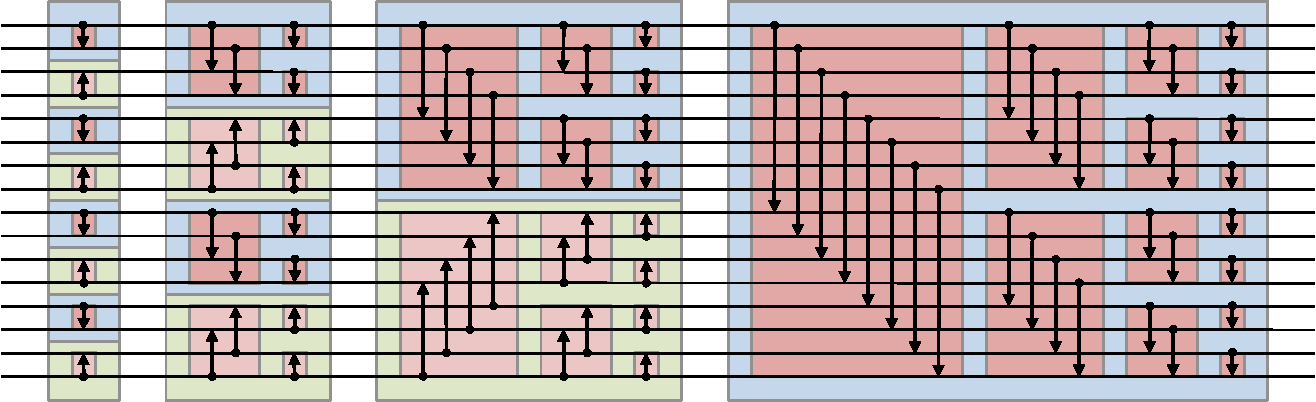
\includegraphics[width=\linewidth]{07/figs/bitonic.pdf}
    \end{center}
    \vspace{0.5em}
    Součástí řazení je i podmíněné prohazování prvků v poli: zjednodušená verze na dalších slidech.
\end{frame}

\begin{frame}[fragile]
  \frametitle{Podmíněné zpracování}

  Občas chceme zpracovat různé prvky různým způsobem...
  \begin{minted}{c}
    size_t half = N / 2;
    for(unsigned int i = 0 ; i < half ; i++) {
        if(data[i] > data[i+half])
          std::swap(data[i], data[i+half]);
    }
  \end{minted}

  \pause
  \vspace{1em}\hrule\vspace{1em}
  \mintinline{c}{__m256 _mm256_blendv_ps(x, y, mask)}:
  \begin{center}
    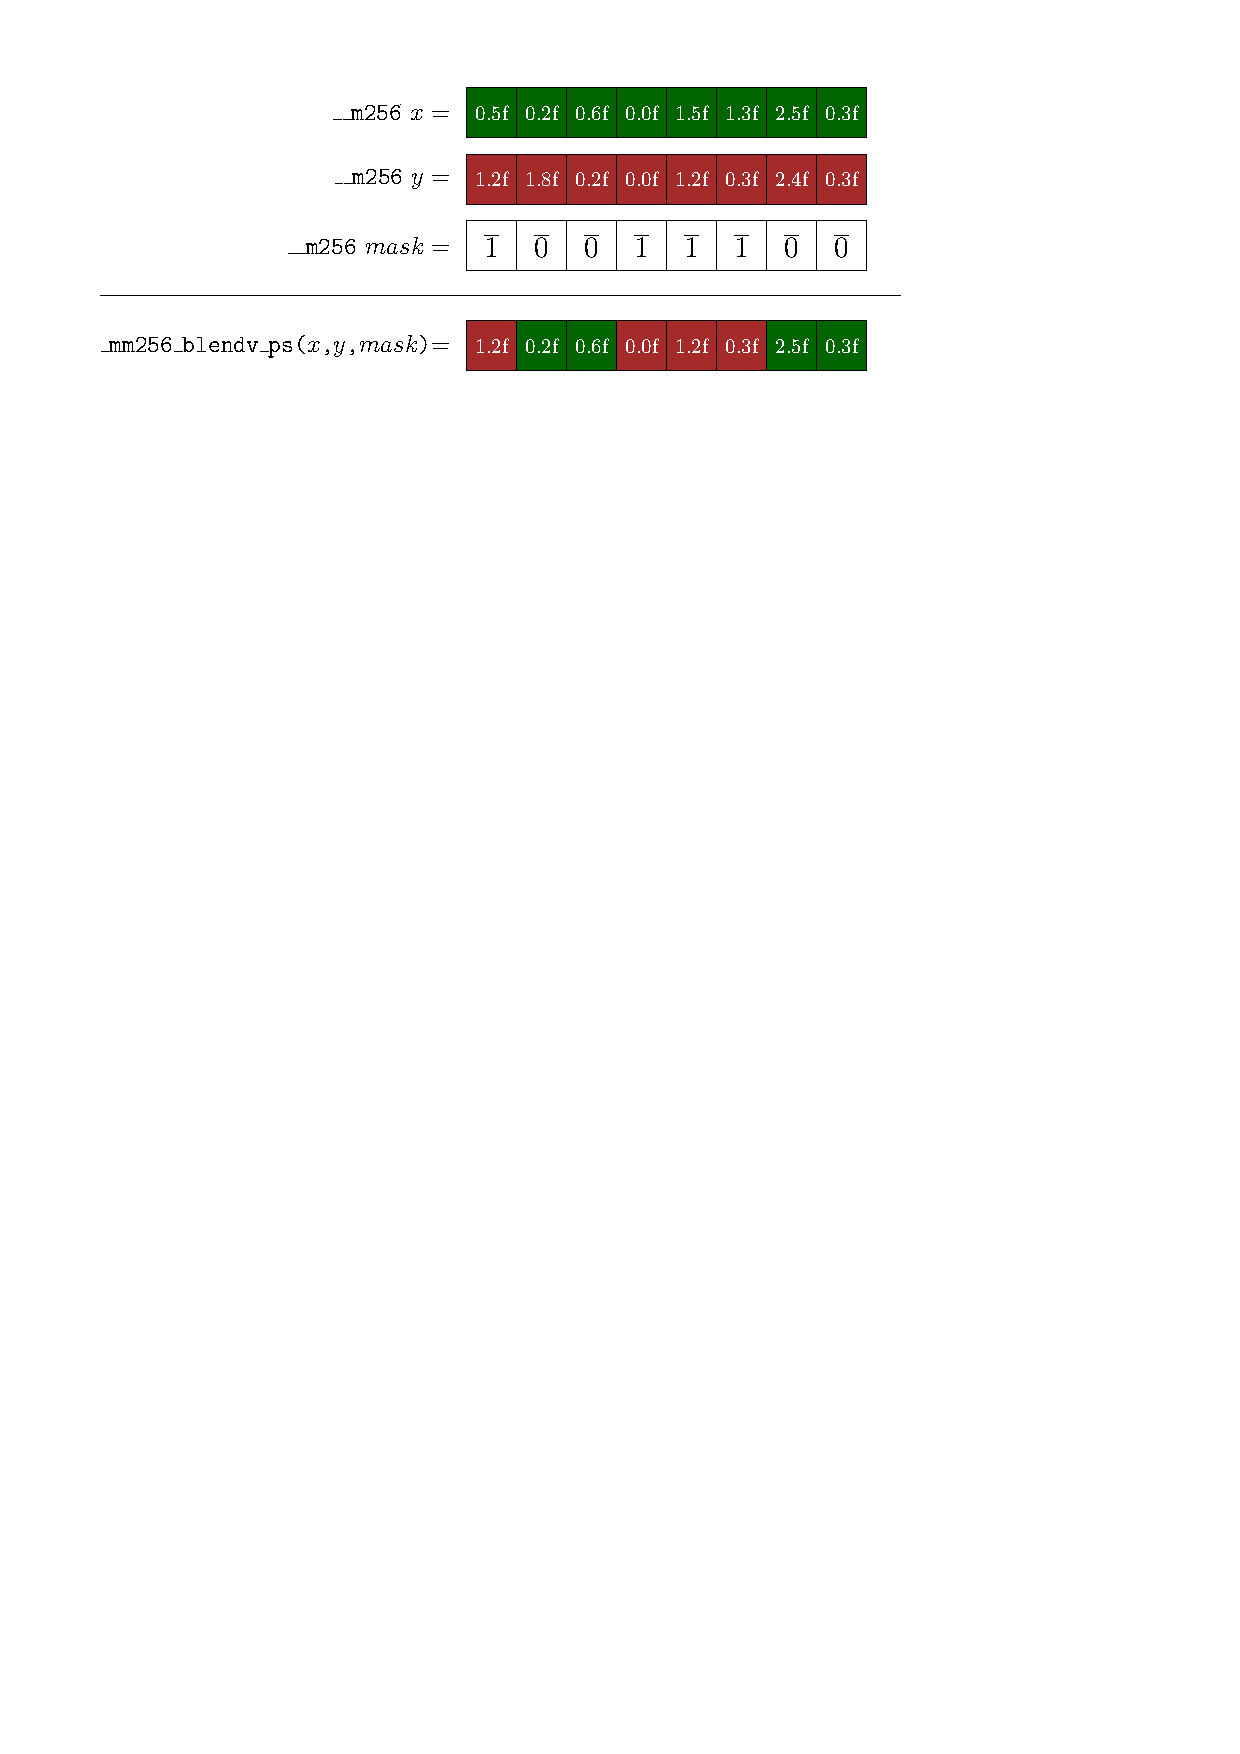
\includegraphics[width=0.95\linewidth]{07/figs/blendv.pdf}
  \end{center}
\end{frame}

{\setbeamertemplate{frame footer}{\exe{{\tt condswap[.exe]}}}
\begin{frame}[fragile]
  \frametitle{Podmíněné zpracování}

  \begin{block}{Doimplementujte tělo metody \texttt{condswap\_vec(...)}}
    Doimplementujte tělo metody \texttt{condswap\_vec(...)} v souboru \texttt{cond.cpp}, která bude vektorově vykonávat následující kód
    \begin{minted}{c}
    size_t half = N / 2;
    for(unsigned int i = 0 ; i < half ; i++) {
        if(data[i] > data[i+half])
          std::swap(data[i], data[i+half]);
    }
    \end{minted}
    Pro implementaci podmínky využijte \mintinline{c}{_mm256_blendv_ps(x,y,mask)}.
  \end{block}

  \vspace{1.5em}

  Vektorová instrukce pro porovnání vektorů $x < y$ typu \emph{packed-single}:
  \mintinline{c}{__m256 _mm256_cmp_ps(x, y, _CMP_LT_OQ)}
\end{frame}
}


\begin{frame}
  \frametitle{Bitové operace}

  \begin{center}
    \Large S primitivními vektorovými instrukcemi jste se setkali už dříve!

    \normalsize například \mintinline{c}{x & y} nebo \mintinline{c}{x ^ y}
  \end{center}

  \vspace{3em}

  \pause
  \hfill My se podíváme na něco zajímavějšího...
\end{frame}

{\setbeamertemplate{frame footer}{\exe{{\tt lzcnt[.exe]}}}
\begin{frame}
  \frametitle{Bitové operace}

  \mintinline{c}{_lzcnt_u64(uint64_t x)} \\
  \mintinline{c}{_tzcnt_u64(uint64_t x)}

  \vspace{-0.35em}\hspace{10pt} Počet \emph{leading}, resp. \emph{trailing zeros} v čísle \texttt{x}

  \vspace{1em}

  Například:

  \hspace{10pt} \mintinline{c}{_lzcnt_u64(0b00001000 ... 00011100) = 4}

  \hspace{10pt} \mintinline{c}{_tzcnt_u64(0b00001000 ... 00011100) = 2}

  \vspace{1em}
  \pause

  \begin{block}{Doimplementujte tělo metody \texttt{log2\_lzcnt(...)}}
    Doimplementujte tělo metody \texttt{log2\_lzcnt(...)} v souboru \texttt{lzcnt.cpp}.
    Pro \texttt{x > 0} má tato metoda provést výpočet ekvivalentní \texttt{(int)log2(x)}.

    Tip: Jaký vztah má pozice nejvyššího jedničkového bitu k hodnotě logaritmu o základu 2?
  \end{block}
\end{frame}
}

{\setbeamertemplate{frame footer}{\exe{{\tt popcnt[.exe]}}}
\begin{frame}
  \frametitle{Bitové operace}

  \mintinline{c}{_mm_popcnt_u64(uint64_t x)}

  \vspace{-0.35em}\hspace{10pt} Počet jedničkových bitů v čísle \texttt{x}
  
  \begin{block}{Doimplementujte tělo metody \texttt{popcnt\_intrinsic(...)}}
    Doimplementujte tělo metody \texttt{popcnt\_intrinsic(...)} v souboru \texttt{popcnt.cpp}.
  \end{block}
\end{frame}
}

\section{Semestrální úloha}

\begin{frame}
  \frametitle{Semestrální úloha}
  \begin{center}
    \Large Prohledávání stavového prostoru
  \end{center}
  
    \vspace{1em}
  
  \begin{center}
  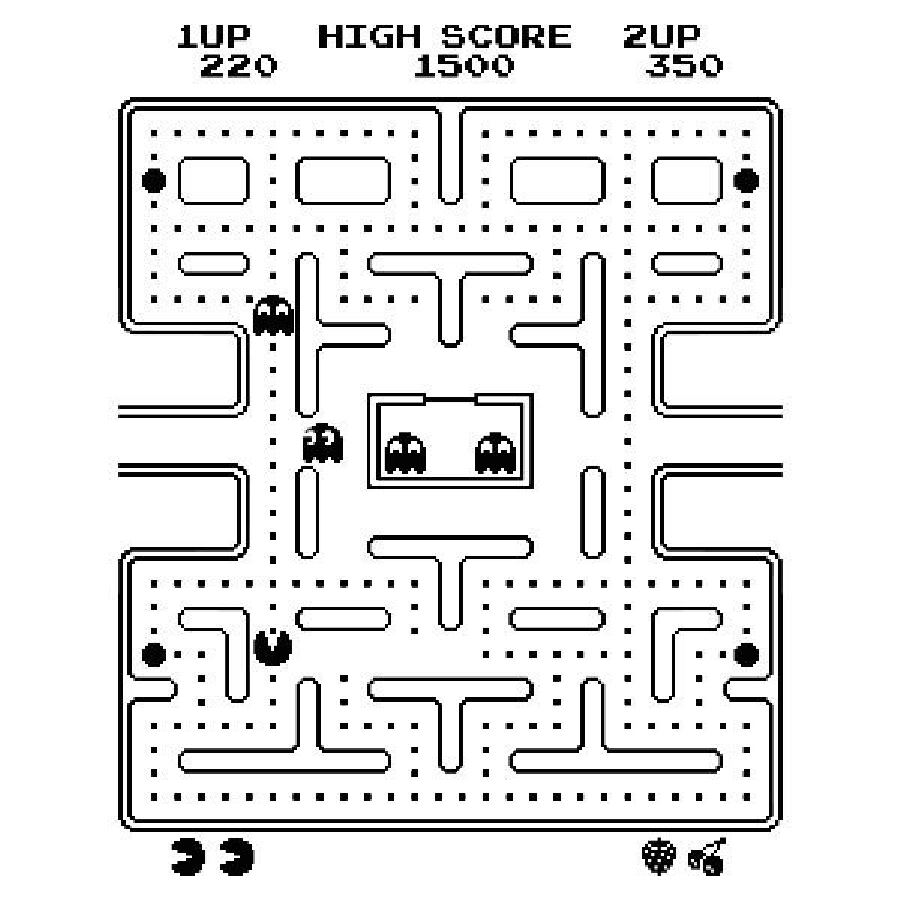
\includegraphics[width=.4\linewidth]{07/figs/pacman2.pdf}
  \end{center}
  
%  \hfill Budeme po vás chtít nejkratší
%
%  \hfill (resp. nejlevnější) cestu v grafu...

  \vspace{2em}

  \hrule
  \begin{center}
  \end{center}
\end{frame}

% Frame with the feedback QR code 
\framefeedback{}

\end{document}
